% !TEX root = ../main.tex
\begin{figure}[t]
\vspace{-0.5in}
\centering
\iflatexml
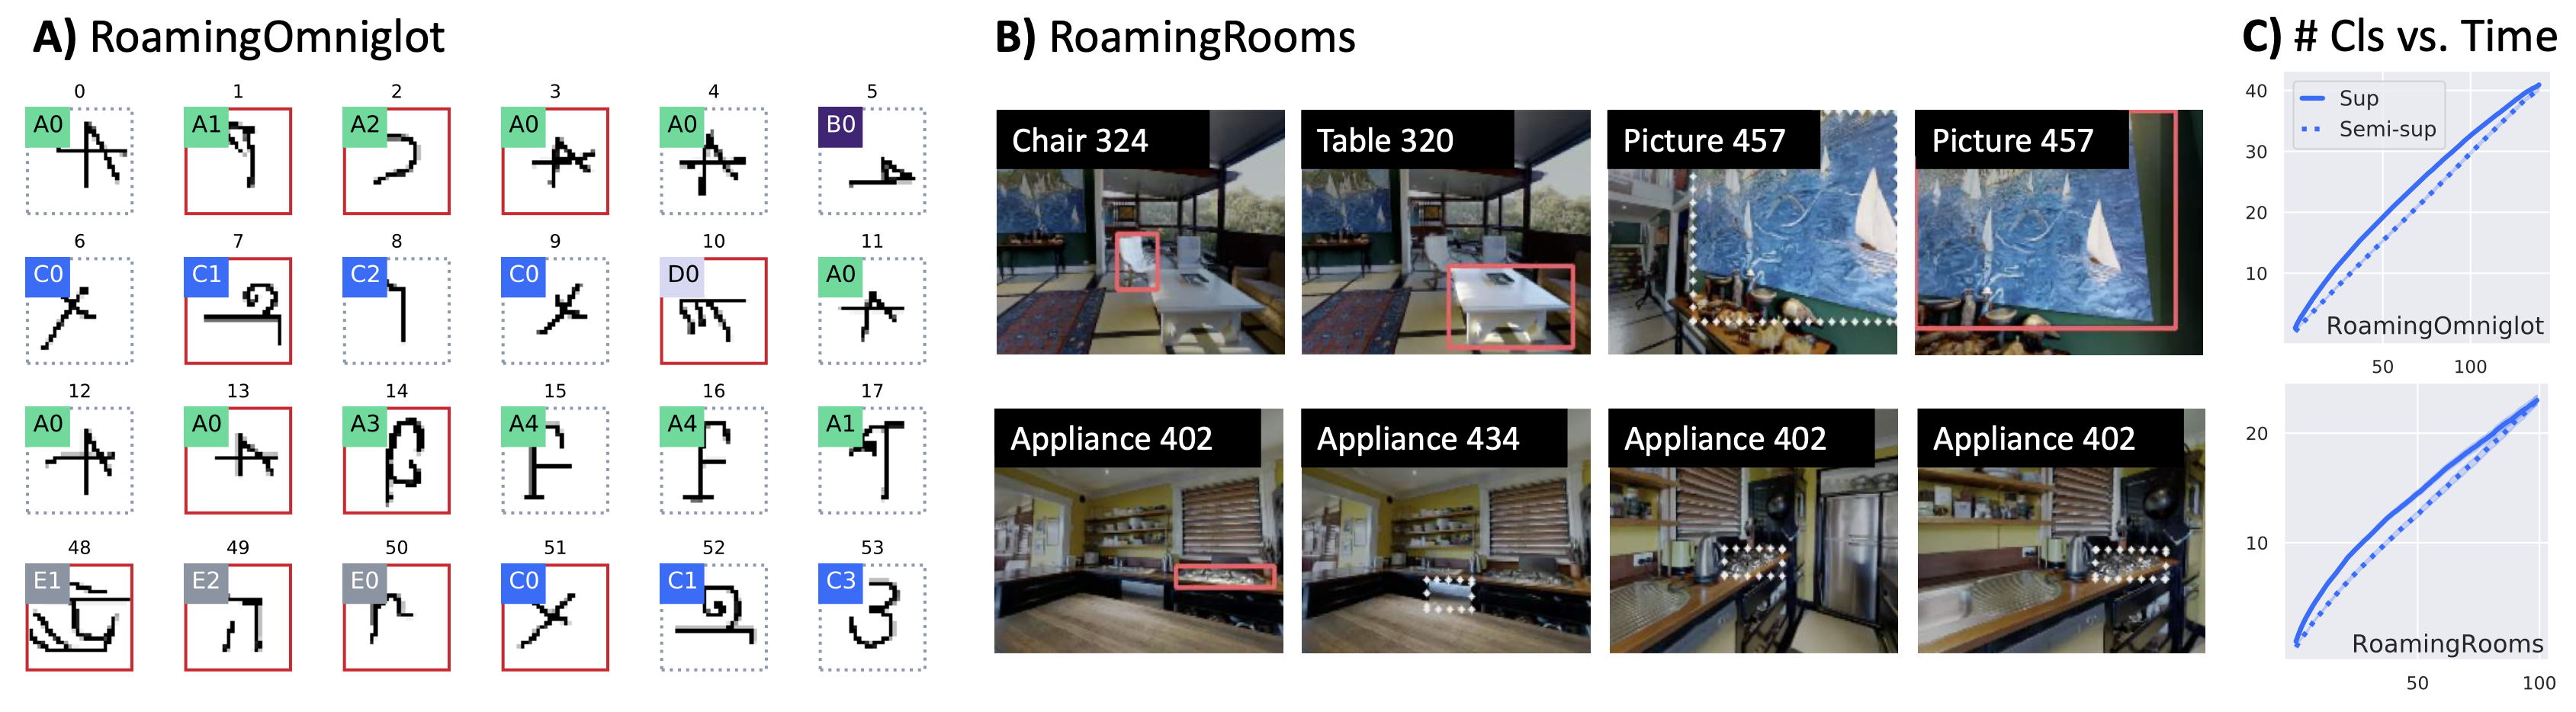
\includegraphics[width=6\textwidth]{figures/datasets-copy-samll-compressed-2.png}
\else
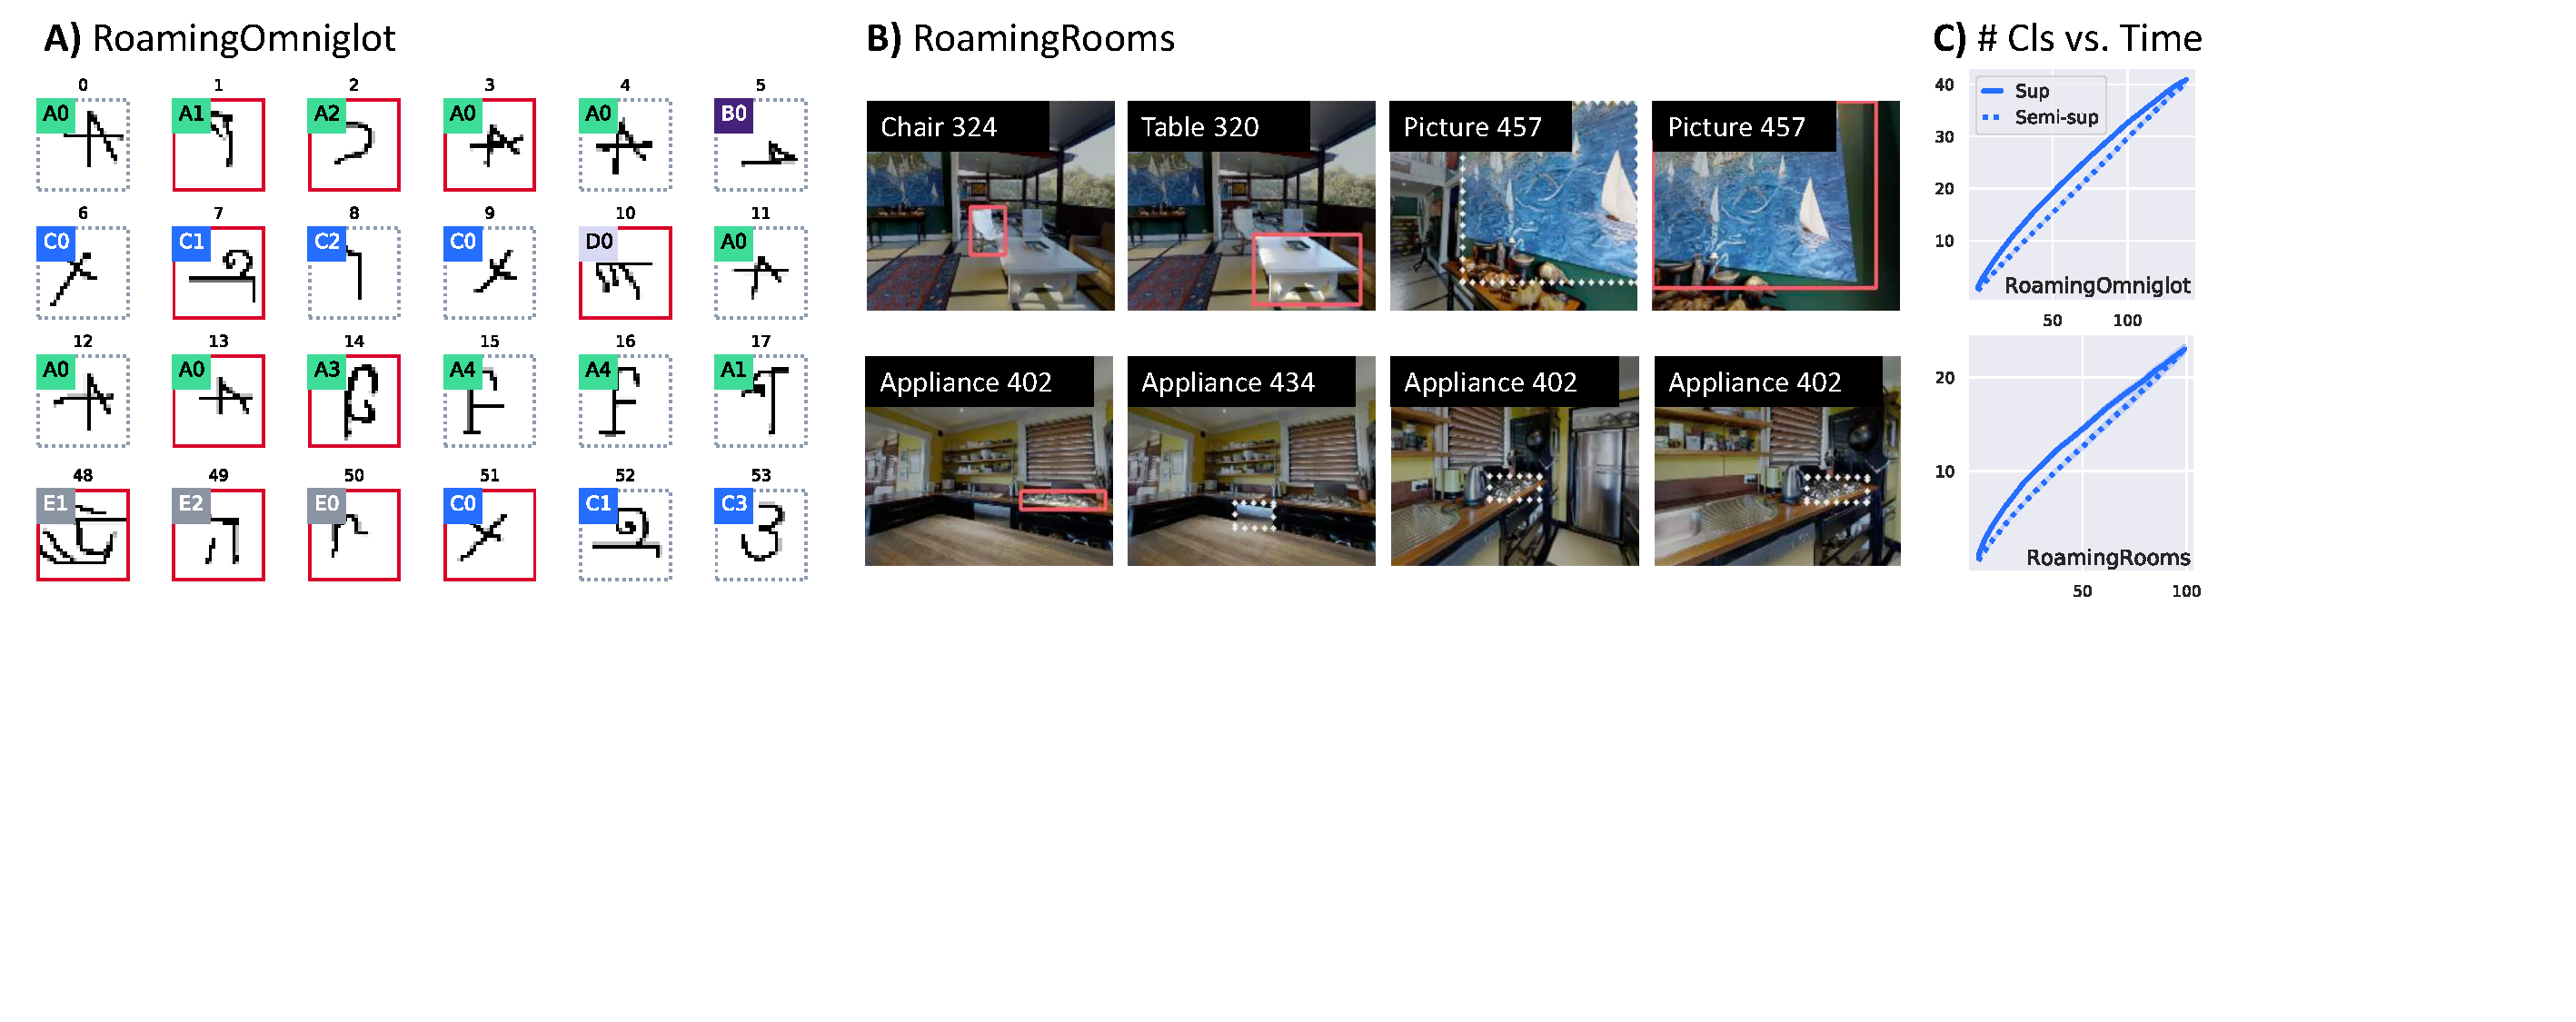
\includegraphics[width=\textwidth, trim={0cm 7cm 6.5cm 0}, clip]{figures/datasets-copy-small-compressed-2.pdf}
\fi
\vspace{-0.32in}
\caption{\looseness=-1 \textbf{Sample online contextualized few-shot learning sequences.} \textbf{A)}
\ourchar{}. Red solid boxes denote labeled examples of Omniglot handwritten characters, and
dotted boxes denote unlabeled ones. Environments are shown in colored labels in the top left corner.
\textbf{B)} Image frame samples of a few-shot learning sequence in our \ourroom{} dataset collected
from a random walking agent. The task here is to recognize and classify novel instance IDs in the home environment. Here the groundtruth instance masks/bounding boxes are provided.
\textbf{C)} The growth of total number of labeled classes in a sequence for \ourchar{} (top) and
\ourroom{} (bottom).}
\label{fig:dataset}
\vspace{-0.15in}
\end{figure}
